% Diagramas en TikZ, uno por página. Compilar: latexmk, desde esta carpeta (el PDF va a figures/slides).
\documentclass[border=16pt,multi=slide]{standalone}
\usepackage[T1]{fontenc}
\usepackage[utf8]{inputenc}
\usepackage[sfdefault]{inter}
\usepackage{tikz}
\usetikzlibrary{arrows.meta,positioning,calc,fit}
\definecolor{ink}{HTML}{111111}
\definecolor{ink2}{HTML}{3C4043}
\definecolor{muted}{HTML}{8A8F98}
\definecolor{rule}{HTML}{D9DBDF}
\definecolor{soft}{HTML}{F4F5F7}
\definecolor{own}{HTML}{E5484D}
\definecolor{starved}{HTML}{F0A530}
\definecolor{blocked}{HTML}{3E8BF0}
\tikzset{
  box/.style={draw=rule, line width=0.8pt, rounded corners=6pt, fill=white, minimum height=17mm, text width=33mm, align=center, inner sep=6pt, font=\small\color{ink2}},
  key/.style={box, draw=ink, line width=1.2pt},
  stepnum/.style={font=\scriptsize\bfseries\color{muted}},
  flow/.style={-{Stealth[length=3mm]}, line width=1pt, color=ink},
  machine/.style={draw=ink, line width=1.2pt, rounded corners=5pt, minimum width=24mm, minimum height=20mm, fill=white, font=\large\bfseries},
}
\begin{document}

% 1 · De los datos a la decisión ------------------------------------------------------------
\begin{slide}
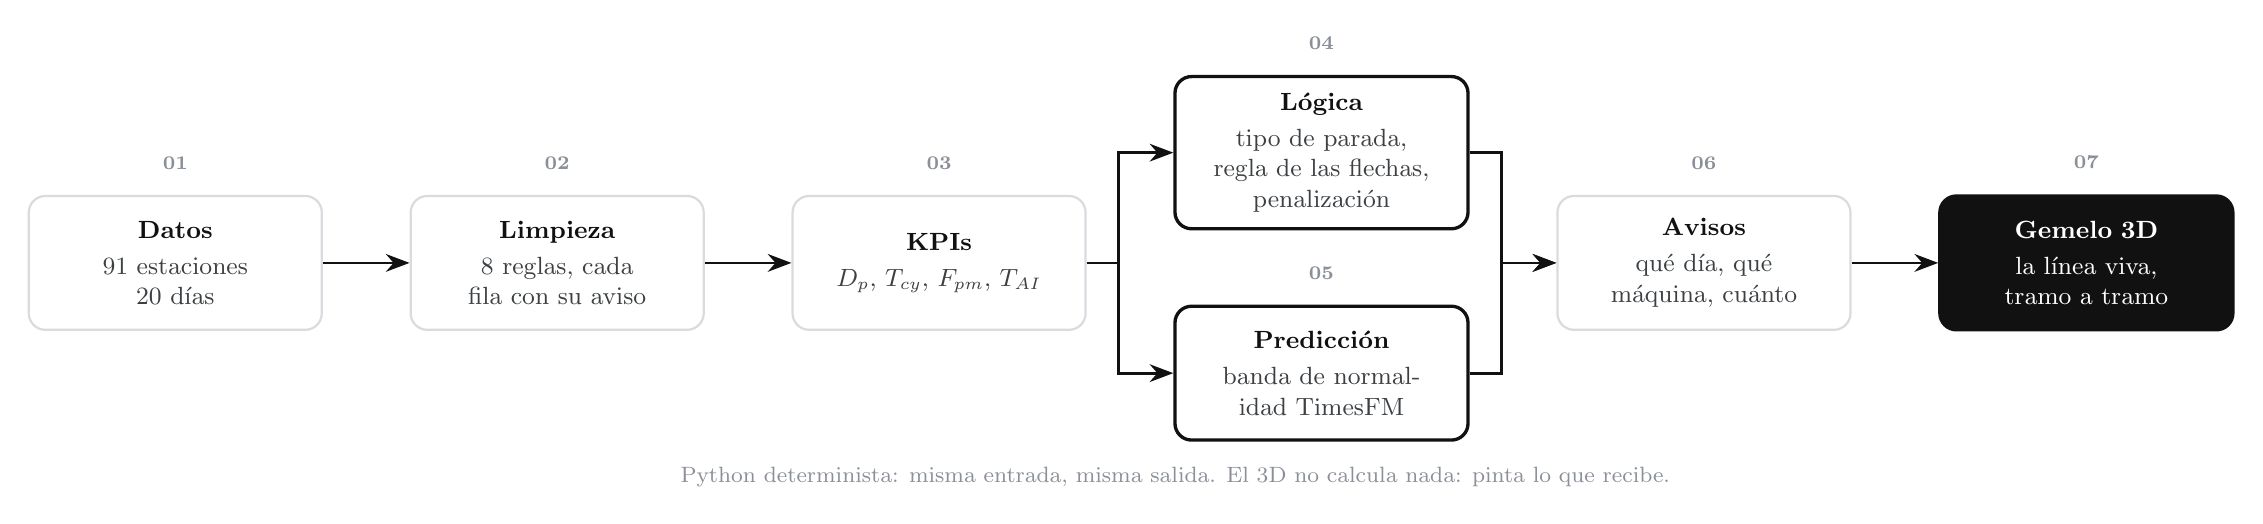
\begin{tikzpicture}[node distance=11mm]
  \node[box] (data) {{\bfseries\color{ink}Datos}\\[2pt]91 estaciones\\20 días};
  \node[box, right=of data] (clean) {{\bfseries\color{ink}Limpieza}\\[2pt]8 reglas, cada fila con su aviso};
  \node[box, right=of clean] (kpi) {{\bfseries\color{ink}KPIs}\\[2pt]$D_p$, $T_{cy}$, $F_{pm}$, $T_{AI}$};
  \node[key, right=of kpi, yshift=14mm] (logic) {{\bfseries\color{ink}Lógica}\\[2pt]tipo de parada, regla de las flechas, penalización};
  \node[key, right=of kpi, yshift=-14mm] (pred) {{\bfseries\color{ink}Predicción}\\[2pt]banda de normalidad TimesFM};
  \node[box, right=of logic, yshift=-14mm] (alerts) {{\bfseries\color{ink}Avisos}\\[2pt]qué día, qué máquina, cuánto};
  \node[key, right=of alerts, fill=ink, text=white] (twin) {{\bfseries Gemelo 3D}\\[2pt]la línea viva, tramo a tramo};
  \draw[flow] (data) -- (clean);
  \draw[flow] (clean) -- (kpi);
  \draw[flow] (kpi.east) -- ++(4mm,0) |- (logic.west);
  \draw[flow] (kpi.east) -- ++(4mm,0) |- (pred.west);
  \draw[flow] (logic.east) -- ++(4mm,0) |- (alerts.west);
  \draw[flow] (pred.east) -- ++(4mm,0) |- (alerts.west);
  \draw[flow] (alerts) -- (twin);
  \node[stepnum, above=2mm of data] {01};
  \node[stepnum, above=2mm of clean] {02};
  \node[stepnum, above=2mm of kpi] {03};
  \node[stepnum, above=2mm of logic] {04};
  \node[stepnum, above=2mm of pred] {05};
  \node[stepnum, above=2mm of alerts] {06};
  \node[stepnum, above=2mm of twin] {07};
  \node[font=\footnotesize\color{muted}, below=16mm of kpi, anchor=north, xshift=30mm] {Python determinista: misma entrada, misma salida. El 3D no calcula nada: pinta lo que recibe.};
\end{tikzpicture}
\end{slide}

% 2 · Regla de las flechas -------------------------------------------------------------------
\begin{slide}
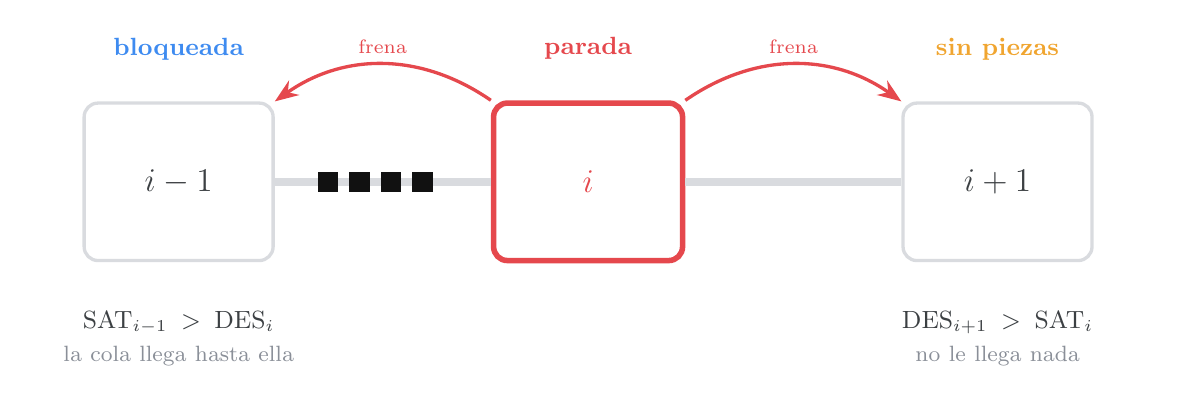
\begin{tikzpicture}
  \node[machine, draw=rule, text=ink2] (a) at (0,0) {$i-1$};
  \node[machine, draw=own, line width=2pt, text=own] (b) at (5.2,0) {$i$};
  \node[machine, draw=rule, text=ink2] (c) at (10.4,0) {$i+1$};
  \draw[line width=3pt, color=rule] (a.east) -- (b.west);
  \draw[line width=3pt, color=rule] (b.east) -- (c.west);
  \foreach \x in {1.9,2.3,2.7,3.1} \fill[ink] (\x-0.13,-0.13) rectangle ++(0.26,0.26);
  \node[font=\small\bfseries, color=blocked, above=4mm of a] {bloqueada};
  \node[font=\small\bfseries, color=own, above=4mm of b] {parada};
  \node[font=\small\bfseries, color=starved, above=4mm of c] {sin piezas};
  \node[font=\small\color{ink2}, below=5mm of a, text width=36mm, align=center] {$\mathrm{SAT}_{i-1} > \mathrm{DES}_i$\\[1pt]{\color{muted}\footnotesize la cola llega hasta ella}};
  \node[font=\small\color{ink2}, below=5mm of c, text width=36mm, align=center] {$\mathrm{DES}_{i+1} > \mathrm{SAT}_i$\\[1pt]{\color{muted}\footnotesize no le llega nada}};
  \draw[-{Stealth[length=3mm]}, line width=1.2pt, color=own] (b.north west) to[bend right=35] node[above, font=\scriptsize\color{own}] {frena} (a.north east);
  \draw[-{Stealth[length=3mm]}, line width=1.2pt, color=own] (b.north east) to[bend left=35] node[above, font=\scriptsize\color{own}] {frena} (c.north west);
\end{tikzpicture}
\end{slide}

% 3 · Topología: el config solo da el orden ---------------------------------------------------
\begin{slide}
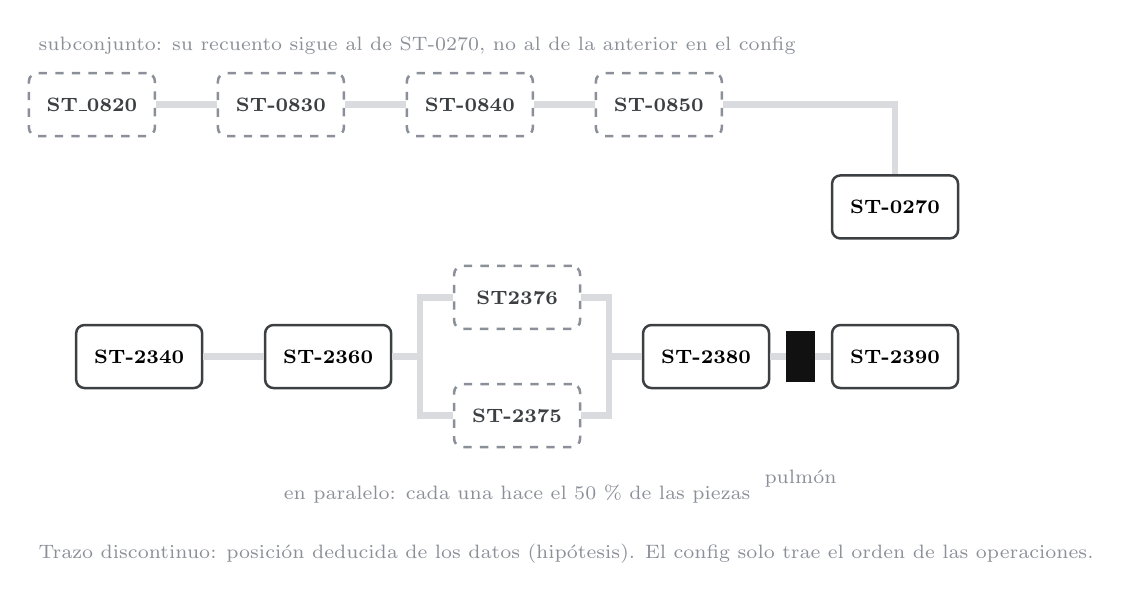
\begin{tikzpicture}[x=1cm,y=1cm]
  \tikzset{st/.style={draw=ink2, line width=0.9pt, rounded corners=3pt, minimum width=16mm, minimum height=8mm, font=\scriptsize\bfseries, fill=white},
           hyp/.style={st, dashed, draw=muted, text=ink2},
           belt/.style={line width=2.4pt, color=rule}}
  % flujo principal
  \foreach \n/\x in {ST-2340/0, ST-2360/2.4, ST-2380/7.2, ST-2390/9.6} \node[st] (\n) at (\x,0) {\n};
  \node[hyp] (p1) at (4.8,0.75) {ST2376};
  \node[hyp] (p2) at (4.8,-0.75) {ST-2375};
  \draw[belt] (ST-2340) -- (ST-2360);
  \draw[belt] (ST-2360.east) -- ++(0.35,0) |- (p1.west);
  \draw[belt] (ST-2360.east) -- ++(0.35,0) |- (p2.west);
  \draw[belt] (p1.east) -- ++(0.35,0) |- (ST-2380.west);
  \draw[belt] (p2.east) -- ++(0.35,0) |- (ST-2380.west);
  \draw[belt] (ST-2380) -- (ST-2390);
  \fill[ink] ($(ST-2380)!0.5!(ST-2390)+(-0.18,-0.32)$) rectangle ++(0.36,0.64);
  \node[font=\scriptsize\color{muted}, below=9mm of ST-2380, xshift=12mm] {pulmón};
  \node[font=\scriptsize\color{muted}, align=center] at (4.8,-1.75) {en paralelo: cada una hace el 50 \% de las piezas};
  % subconjunto
  \node[hyp] (a1) at (-0.6,3.2) {ST\_0820};
  \node[hyp] (a2) at (1.8,3.2) {ST-0830};
  \node[hyp] (a3) at (4.2,3.2) {ST-0840};
  \node[hyp] (a4) at (6.6,3.2) {ST-0850};
  \node[st] (j) at (9.6,1.9) {ST-0270};
  \draw[belt] (a1) -- (a2); \draw[belt] (a2) -- (a3); \draw[belt] (a3) -- (a4);
  \draw[belt] (a4.east) -| (j.north);
  \node[font=\scriptsize\color{muted}, anchor=west] at (-1.4,3.95) {subconjunto: su recuento sigue al de ST-0270, no al de la anterior en el config};
  \node[font=\scriptsize\color{muted}, anchor=west] at (-1.4,-2.5) {Trazo discontinuo: posición deducida de los datos (hipótesis). El config solo trae el orden de las operaciones.};
\end{tikzpicture}
\end{slide}

\end{document}
